\documentclass{standalone}
\usepackage{tikz}

\usetikzlibrary{automata,positioning,arrows,shapes,decorations,calc,
arrows.meta,fit}
\usetikzlibrary{decorations.pathmorphing}
\usetikzlibrary{decorations.pathreplacing}
\usetikzlibrary{decorations.shapes}
\usetikzlibrary{decorations.text}
\usetikzlibrary{decorations.markings}
\usetikzlibrary{decorations.fractals}
\usetikzlibrary{decorations.footprints}

\tikzset{
roundnode/.style={circle, draw=black, very thick, minimum size=20mm},
>={Latex[width=2mm,length=2mm]},
goal/.style={circle, double, draw=black, very thick, minimum size=5mm},
simple/.style={circle, draw=black, very thick, minimum size=20mm},
table/.style={circle, draw=black, very thick, minimum size=20mm, fill=lightgray},
screen/.style={circle, draw=black, very thick, minimum size=20mm, fill=green},
>={Latex[width=2mm,length=2mm]},
base/.style = {rectangle, rounded corners, draw=black,
                         minimum width=4cm, minimum height=1cm,
                         text centered, font=\sffamily},
}

\begin{document}
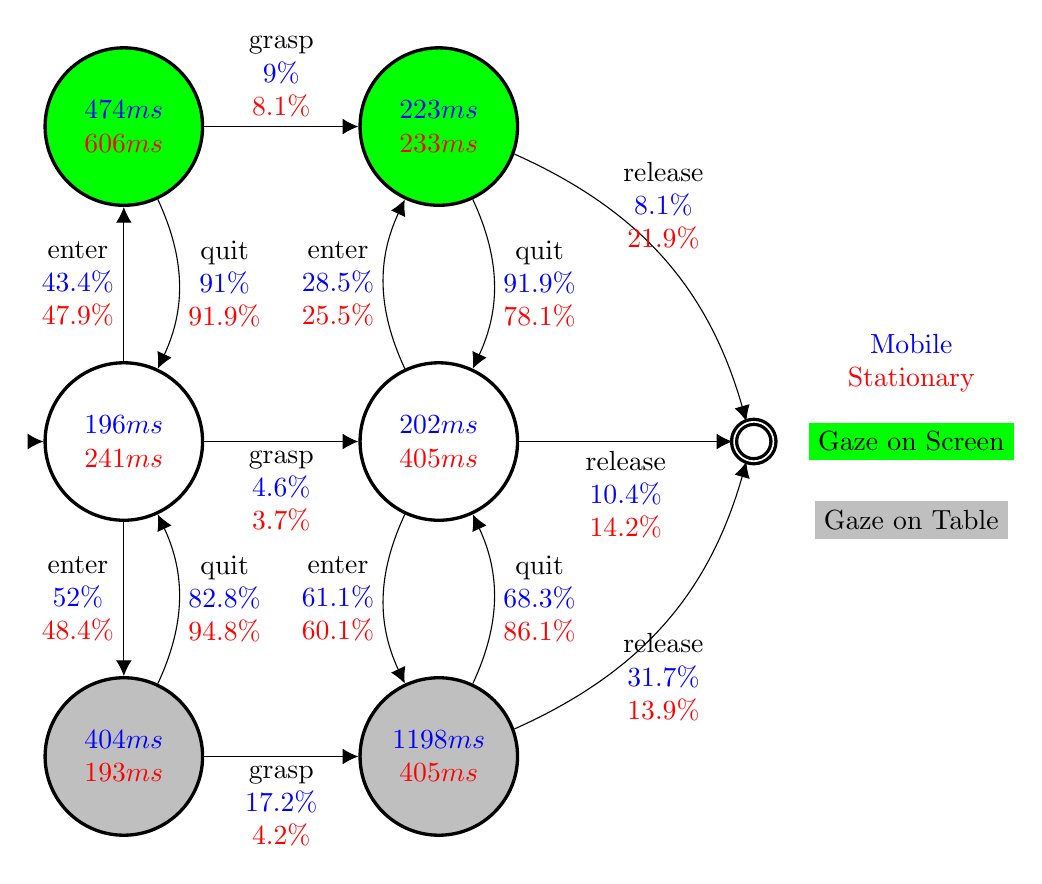
\begin{tikzpicture}[node distance=5cm, align=center]

    \node (start) at(19,-15)  {};

    \node[rectangle] (leg1) at(30, -14)  {\textcolor{blue}{Mobile}\\\textcolor{red}{Stationary}};
    \node[rectangle,fill=green] (leg1) at(30, -15)  {Gaze on Screen};
    \node[rectangle,fill=lightgray] (leg1) at(30, -16)  {Gaze on Table};

    \node[simple] (NO_DEVICE_0) at(20, -15)  {\textcolor{blue}{$196ms$}\\\textcolor{red}{$241ms$}};
    \node[simple] (NO_DEVICE_1) at(24, -15)  {\textcolor{blue}{$202ms$}\\\textcolor{red}{$405ms$}};

    \node[goal] (end) at(28, -15)  {};

    \node[table] (TABLE_0) at(20, -19)  {\textcolor{blue}{$404ms$}\\\textcolor{red}{$193ms$}};
    \node[table] (TABLE_1) at(24, -19)  {\textcolor{blue}{$1198ms$}\\\textcolor{red}{$405ms$}};

    \node[screen] (SCREEN_O) at(20, -11)  {\textcolor{blue}{$474ms$}\\\textcolor{red}{$606ms$}};
    \node[screen] (SCREEN_1) at(24, -11)  {\textcolor{blue}{$223ms$}\\\textcolor{red}{$233ms$}};

    \draw[->] (start)  to (NO_DEVICE_0) ;

    \draw[->] (NO_DEVICE_0)  to node[left] {enter\\\textcolor{blue}{$52\%$}\\\textcolor{red}{$48.4\%$}} (TABLE_0) ;
    \draw[->] (NO_DEVICE_0)  to node[left] {enter\\\textcolor{blue}{$43.4\%$}\\\textcolor{red}{$47.9\%$}} (SCREEN_O) ;
    \draw[->] (NO_DEVICE_0)  tonode[below] {grasp\\\textcolor{blue}{$4.6\%$}\\\textcolor{red}{$3.7\%$}} (NO_DEVICE_1) ;

    \draw[->] (TABLE_0)  to [bend right=25] node[right] {quit\\\textcolor{blue}{$82.8\%$}\\\textcolor{red}{$94.8\%$}} (NO_DEVICE_0) ;
    \draw[->] (TABLE_0)  tonode[below] {grasp\\\textcolor{blue}{$17.2\%$}\\\textcolor{red}{$4.2\%$}} (TABLE_1) ;

    \draw[->] (SCREEN_O)  tonode[above] {grasp\\\textcolor{blue}{$9\%$}\\\textcolor{red}{$8.1\%$}} (SCREEN_1) ;
    \draw[->] (SCREEN_O)  to [bend left=25] node[right] {quit\\\textcolor{blue}{$91\%$}\\\textcolor{red}{$91.9\%$}} (NO_DEVICE_0) ;

    \draw[->] (NO_DEVICE_1)  to node[below] {release\\\textcolor{blue}{$10.4\%$}\\\textcolor{red}{$14.2\%$}} (end) ;
    \draw[->] (TABLE_1)  to [bend left=-25] node[below] {release\\\textcolor{blue}{$31.7\%$}\\\textcolor{red}{$13.9\%$}} (end) ;
    \draw[->] (SCREEN_1)  to [bend left=25] node[above] {release\\\textcolor{blue}{$8.1\%$}\\\textcolor{red}{$21.9\%$}} (end) ;

    \draw[->] (TABLE_1)  to [bend right=25] node[right] {quit\\\textcolor{blue}{$68.3\%$}\\\textcolor{red}{$86.1\%$}} (NO_DEVICE_1) ;
    \draw[->] (SCREEN_1)  to [bend left=25] node[right] {quit\\\textcolor{blue}{$91.9\%$}\\\textcolor{red}{$78.1\%$}} (NO_DEVICE_1) ;

    \draw[->] (NO_DEVICE_1)  to [bend right=25] node[left] {enter\\\textcolor{blue}{$61.1\%$}\\\textcolor{red}{$60.1\%$}} (TABLE_1) ;
    \draw[->] (NO_DEVICE_1)  to [bend left=25] node[left] {enter\\\textcolor{blue}{$28.5\%$}\\\textcolor{red}{$25.5\%$}} (SCREEN_1) ;
\end{tikzpicture}
\end{document}
